%================================================
%	PACKAGES AND THEMES
%================================================
\documentclass[aspectratio=169,xcolor=dvipsnames]{beamer}

\usetheme{SimplePlusAIC}

\usepackage{hyperref}
\usepackage{graphicx} % Allows including images
\usepackage{booktabs} % Allows the use of \toprule, \midrule and  \bottomrule in tables
\usepackage{svg} % Allows using svg figures
\usepackage{tikz}
\usepackage{makecell}
\newcommand*{\defeq}{\stackrel{\text{def}}{=}}
\usepackage{setspace}
\usepackage[T1]{fontenc}
\usepackage[french]{babel}
\usepackage{helvet}
\usepackage{textgreek}
\usepackage{amsmath,amssymb}
\usepackage{bm}
\usepackage{ragged2e}
\usepackage{xfrac}
% \usepackage[nice]{nicefrac}
\usepackage[loose]{units}
\usepackage{braket}
\usepackage{physics}
\usepackage{gensymb}

\usepackage{verbatim}
\usepackage{fancyvrb}
\usepackage{diagbox}

\usetikzlibrary{arrows}
\usetikzlibrary[patterns]

%-- For subfigures
\usepackage{subcaption}

%\setbeamertemplate{blocks}[rounded][shadow] % block options

\usepackage[svgnames,table]{xcolor}
\arrayrulecolor{black}
\setlength{\arrayrulewidth}{0.20mm}
\renewcommand{\arraystretch}{1.40}  % stretch tables row size

\usepackage{blkarray}
\usepackage{dsfont}

\usepackage{eurosym}
\usepackage{multicol}

%================================================
% MATH COMMANDS
%================================================
\newcommand{\R}{\mathbb{R}}
\renewcommand{\P}{\mathbb{P}}
\newcommand\indep{\protect\mathpalette{\protect\independenT}{\perp}}
\def\independenT#1#2{\mathrel{\rlap{$#1#2$}\mkern2mu{#1#2}}}

\newcommand{\argmin}{argmin}
%================================================
% Stuff for R code
%================================================

\usepackage{minted}
%================================================
% Pause après équation
%================================================
\newcommand{\pauseq}{\vspace*{-\baselineskip}\pause}
%================================================
% FontAwesome
\usepackage{fontawesome5}
%================================================

%================================================
%	TITLE PAGE
%================================================
\title[short title]{EC 551 : Statistique descriptive et décisionnelle} 
%\subtitle{Subtitle}

\author[Surname]{Guillaume Franchi}
\institute[CBI]{Cursus Ingénieur $1^{\text{ère}}$ année}

\date{\textcolor{nyublue}{Partie 1 : Statistique descriptive}}


%================================================
%	BEGIN DOCUMENT 
%================================================



\begin{document}

%------------------------------------------------
%	TITLE SLIDE
%------------------------------------------------
\begin{frame}[plain]

    \titlepage
    
\end{frame}

%------------------------------------------------
%	OUTLINE SLIDE
%------------------------------------------------
%\begin{frame}[plain]
%
%    \frametitle{Plan du cours} 
%    %\framesubtitle{~}
%
%    \begin{spacing}{1.2}
%        \tableofcontents[hideallsubsections]
%    \end{spacing}
%    
%\end{frame}
%------------------------------------------------
%	SLIDE PRE-REQUIS
%------------------------------------------------

\begin{frame}[plain]

\textcolor{nyubluedarker}{{\Large \faCogs \ \textbf{Pré-requis}}}
	\begin{itemize}
	\item Connaissances sur le logiciel R (EC 551)
	\end{itemize}
	
	\bigskip
	
\textcolor{nyubluedarker}{{\Large \faBook \ \textbf{Bibiliographie}}}
		\begin{itemize}
	\item  \underline{R pour la statistique et la science des données}, \textit{François Husson et al.}, Presses Universitaires de Rennes.
	\item \underline{Probabilités, Analyse des données et Statistique}, \textit{Gilbert Saporta}, Editions Technip.
	\end{itemize}

\end{frame}

%------------------------------------------------
%	NEW SLIDE
%------------------------------------------------
\begin{frame}[plain]
\textcolor{nyubluedarker}{{\Large \faBullseye \ \textbf{Objectifs}}}
	\begin{itemize}
	\item Présenter, décrire et résumer des données nombreuses et variées issues de phénomènes économiques, physiques ou biologiques.
	\item Mettre en \oe{}uvre des techniques d'estimation et de test afin de prendre la meilleure décision possible.
	\end{itemize}
	
	\medskip
	
	\textcolor{nyubluedarker}{{\Large \faChalkboardTeacher \ \textbf{Enseignement}}}
	\begin{itemize}
	\item Partie 1 : Statistique descriptive (G. Franchi - 2CMs, 4TDs).
	\item Partie 2 : Statistique inférentielle (M.Semenou - 1CM, 12 TDs).
	\end{itemize}	
	
	\medskip

\textcolor{nyubluedarker}{{\Large \faGraduationCap \ \textbf{Modalités d'évaluation}}}
	\begin{itemize}
	\item 1 évaluation écrite (2h - coefficient 2) commune aux deux parties.
	\item 1 Projet couplé avec l'EC 552 - Introduction au langage R (coefficient 1).
	\end{itemize}

\end{frame}


%~~~~~~~~~~~~~~~~~~~~~~~~~~~~~~~~~~~~~~~~~~~~~~~~
\section{Introduction}
%~~~~~~~~~~~~~~~~~~~~~~~~~~~~~~~~~~~~~~~~~~~~~~~~

%------------------------------------------------
%	NEW SLIDE
%------------------------------------------------
\begin{frame}[plain]

\vfill

\begin{center}
{\huge \textcolor{nyubluedark}{\textbf{1. Introduction}}}
\end{center}

\vfill

\end{frame}

%------------------------------------------------
%	NEW SLIDE
%------------------------------------------------
\begin{frame}

\begin{block}{\textbf{Définition}}

La \textbf{statistique} désigne à la fois un ensemble de données d'observations, et l'activité qui consiste dans
	\begin{itemize}
	\item leur recueil,
	\item leur traitement,
	\item et leur interprétation. \hfill \emph{(Encyclopedia Universalis)}
	\end{itemize}

\end{block}

\begin{exampleblock}{\textbf{Remarque}}
En \textbf{statistique descriptive}, on s'intéressera essentiellement à résumer l'information contenue dans les données de façon synthétique et efficace :
	\begin{itemize}
	\item par des représentations graphiques;
	\item par des indicateurs statistiques \emph{(statistiques univariées)};
	\item par des relations entre les variables \emph{(statistiques multivariées)}.
	\end{itemize}
\end{exampleblock}

\end{frame}

%------------------------------------------------
%	NEW SLIDE
%------------------------------------------------
\begin{frame}

	\begin{exampleblock}{\textbf{Exemple}}

	Une enseigne de salles de sport a interrogé 973 de ces clients afin de mieux déterminer le \og profil-type \fg{} des usagers. On présente ici quelques données récoltées.

		\begin{center}
		\begin{tabular}{rrllrrr}
  \hline
 & Age & Sexe & Type & Taille(m) & Poids(kg) & Volume\_hebdo(h) \\ 
  \hline
1 &  56 & Feminin & Yoga & 1.71 & 60.30 & 6.76 \\ 
  2 &  46 & Feminin & HIIT & 1.53 & 44.50 & 5.20 \\ 
  3 &  32 & Masculin & Cardio & 1.66 & 68.10 & 4.44 \\ 
  4 &  25 & Masculin & Force & 1.70 & 73.20 & 1.77 \\ 
  5 &  38 & Feminin & Force & 1.69 & 66.10 & 1.92 \\ 
  6 &  56 & Feminin & HIIT & 1.68 & 58.00 & 7.95 \\ 
   \hline
		\end{tabular}
		\end{center}

	\end{exampleblock}

\end{frame}

%------------------------------------------------
%	NEW SLIDE
%------------------------------------------------
\begin{frame}
	\begin{exampleblock}{\textbf{Exemple (suite)}}
	\begin{itemize}
	\item Si on s'intéresse au temps passé par les clients dans la salle de sport, on peut représenter un histogramme ou un boxplot.
		\begin{figure}
		\centering
		\begin{subfigure}{0.48\linewidth}
		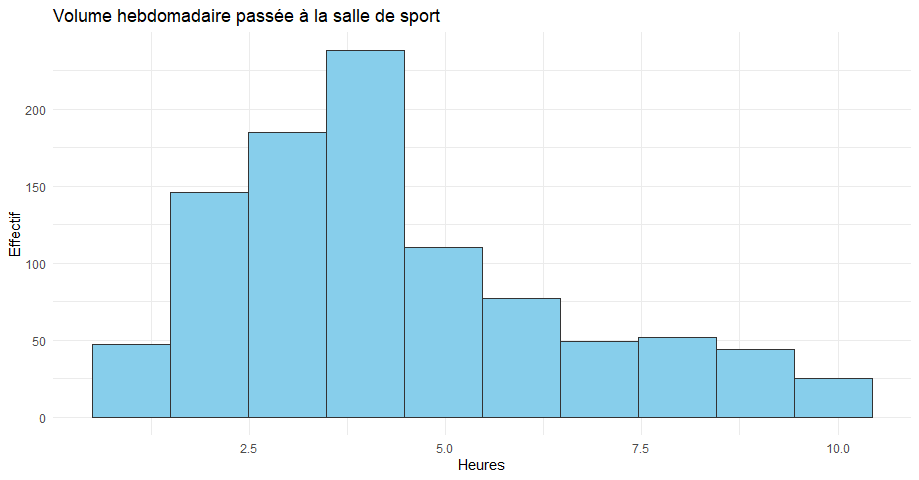
\includegraphics[scale=0.25]{histo_gym1.png}
		\end{subfigure}
		\begin{subfigure}{0.48\linewidth}
		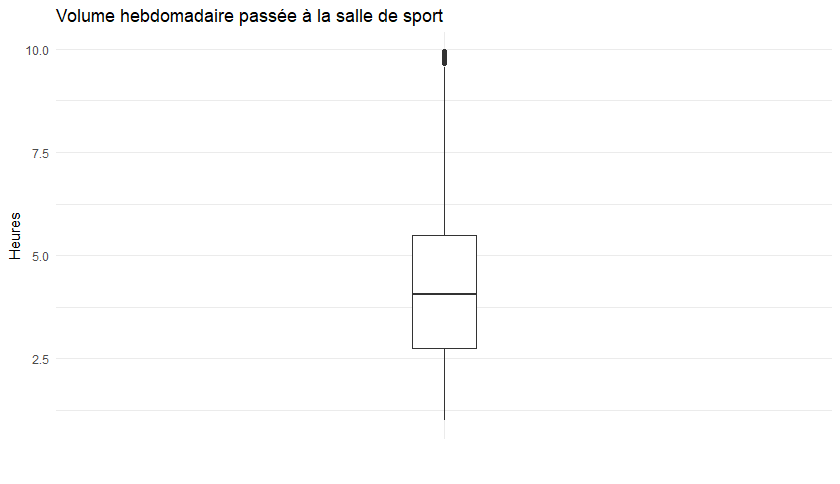
\includegraphics[scale=0.25]{boxplot_gym1.png}
		\end{subfigure}
		\end{figure}
	\item Quelques indicateurs statistiques de cette variable:
		\begin{itemize}
		\item Moyenne : 4.375.
		\item Médiane : 4.050.
		\item Quartiles : $Q_1=2.760$ et $Q_3 = 5.480$.
		\end{itemize}
	\end{itemize}
	\end{exampleblock}
\end{frame}

%------------------------------------------------
%	NEW SLIDE
%------------------------------------------------
\begin{frame}
	\begin{exampleblock}{\textbf{Exemple (suite)}}
\begin{footnotesize}
		\begin{itemize}
		\item On peut aussi s'intéresser au lien entre les deux variables catégorielles : \og Sexe \fg{} et \og Type \fg{}.

			\begin{center}
			\begin{tabular}{rrrrr}
  \hline
 & Cardio & HIIT & Force & Yoga \\ 
  \hline
Masculin & 117 & 117 & 170 &  34 \\ 
  Feminin & 138 & 104 &  88 & 205 \\ 
   \hline
			\end{tabular}
			\end{center}
		
			\begin{center}
			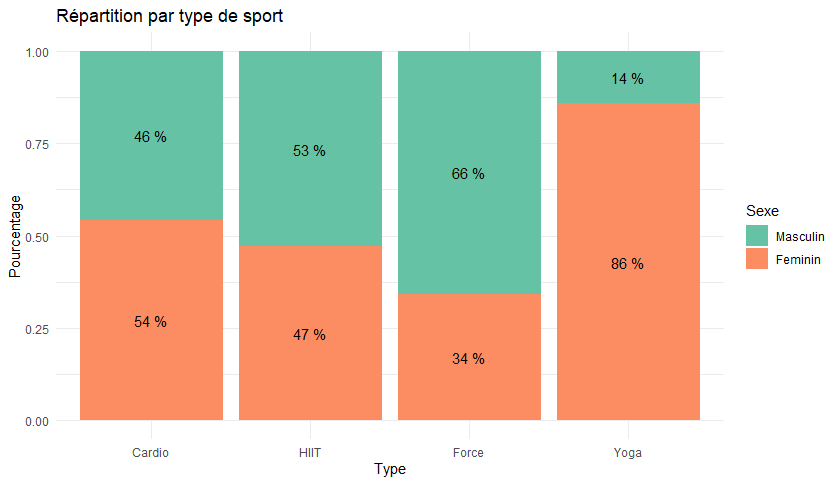
\includegraphics[scale=0.35]{barplot_gym1.png}
			\end{center}
		\end{itemize}
\end{footnotesize}
	\end{exampleblock}
\end{frame}

%------------------------------------------------
%	NEW SLIDE
%------------------------------------------------
\begin{frame}
	\begin{block}{\textbf{Population vs Echantillon}}
		\begin{itemize}
		\item En statistique, une \textbf{population} désigne un ensemble d'\textbf{individus} ayant des propriétés communes. Ces propriétés sont décrites par des \textbf{variables}.
		\item L'étude de tous les individus de la population s'appelle un \textbf{recensement}.
		\item En général, un recensement de la population est impossible et on n'observe qu'une partie de la population, appelée \textbf{échantillon}.
		\end{itemize}
	\begin{center}
	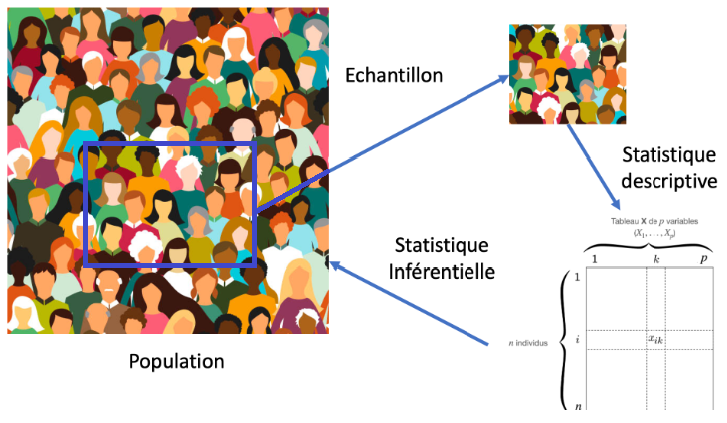
\includegraphics[scale=0.32]{pop_vs_sample.png}
	\end{center}
	\end{block}
\end{frame}

%------------------------------------------------
%	NEW SLIDE
%------------------------------------------------
\begin{frame}

	\begin{block}{\textbf{Base de données}}
\begin{footnotesize}
	Les données recueillies en statistique se présentent toujours sous la forme d'un tableau.
		\begin{itemize}
		\item Les colonnes du tableau représentent les variables (ou caractéristiques) étudiées dans la population.
		\item Les lignes du tableau représentent les individus qui ont été sélectionnés dans l'échantillon.
		\end{itemize}
\end{footnotesize}
	\end{block}
	
	\begin{exampleblock}{\textbf{Exemple}}
\begin{footnotesize}
	Dans le cas de l'enseigne de salles de sport, il serait trop long et onéreux d'interroger la totalité des clients. On se contente donc d'en interroger un échantillon de 973 personnes :
			\begin{center}
		\begin{tabular}{rrllrrr}
  \hline
Individu & Age & Sexe & Type & Taille(m) & Poids(kg) & Volume\_hebdo(h) \\ 
  \hline
1 &  56 & Feminin & Yoga & 1.71 & 60.30 & 6.76 \\ 
  2 &  46 & Feminin & HIIT & 1.53 & 44.50 & 5.20 \\ 
  3 &  32 & Masculin & Cardio & 1.66 & 68.10 & 4.44 \\ 
  4 &  25 & Masculin & Force & 1.70 & 73.20 & 1.77 \\ 
  5 &  38 & Feminin & Force & 1.69 & 66.10 & 1.92 \\ 
   \hline
		\end{tabular}
		\end{center}
\end{footnotesize}
	\end{exampleblock}
\end{frame}

%------------------------------------------------
%	NEW SLIDE
%------------------------------------------------
\begin{frame}
	\begin{block}{\textbf{Types de variables}}
	On distingue deux grandes familles de variables :
		\begin{itemize}
		\item Les \textbf{variables qualitatives} : elles correspondent à un ensemble de catégories \emph{(ou classes)} auxquelles peut appartenir un individu.
		\item Les \textbf{variables quantitatives} : elles décrivent un individu de façon numérique, selon une échelle ordonnée.
		\end{itemize}
	\end{block}
	
	\medskip
	
	\begin{exampleblock}{\textbf{Remarque}}
	Les classes \emph{(ou \textbf{modalités})} d'une variable qualitative peuvent être codées de façon numérique. Elles ne sont pas pour autant des variables quantitatives.
	\end{exampleblock}
\end{frame}

%------------------------------------------------
%	NEW SLIDE
%------------------------------------------------
\begin{frame}
	\begin{block}{\textbf{Echelles de mesure}}
		\begin{center}
		\begin{tabular}{ccc}
		\textbf{Type Variable} & \textbf{Type Données} & \textbf{Exemple} \\
		\hline
		Qualitative & Nominale & Sexe, Type de sport \\
		Qualitative & Ordinale & Niveau, noté de 1 \emph{(Débutant)} à 4 \emph{(Confirmé)} \\
		Quantitative & Discrète & Nombre de séances hebdomadaires \\
		Quantitative & Continue & Poids \\
		\hline 
		\end{tabular}
		\end{center}
	\end{block}
\end{frame}

%~~~~~~~~~~~~~~~~~~~~~~~~~~~~~~~~~~~~~~~~~~~~~~~~
\section{Variables qualitatives}
%~~~~~~~~~~~~~~~~~~~~~~~~~~~~~~~~~~~~~~~~~~~~~~~~

%------------------------------------------------
%	NEW SLIDE
%------------------------------------------------
\begin{frame}[plain]

\vfill

\begin{center}
{\huge \textcolor{nyubluedark}{\textbf{2. Variables qualitatives}}}
\end{center}

\vfill

\end{frame}

%------------------------------------------------
%	NEW SLIDE
%------------------------------------------------
\begin{frame}

	\begin{block}{\textbf{Résumé d'une variable qualitative}}
	Une variable qualitative peut être résumée :
		\begin{itemize}
		\item En comptant, pour chaque modalité $i$, l'\textbf{effectif} $n_i$ des individus appartenant à la modalité $i$.
		\item En calculant, pour chaque modalité $i$, la \textbf{fréquence} $f_i$ des individus appartenant à la modalité $i$. Ici
			\[f_i = \frac{n_i}{N},\]
		$N$ étant l'effectif total de l'échantillon observé.
		\end{itemize}
	\end{block}

\end{frame}

%------------------------------------------------
%	NEW SLIDE
%------------------------------------------------
\begin{frame}
	\begin{exampleblock}{\textbf{Exemple}}
	Dans le cas des 973 clients interrogés dans des salles de sport, on peut résumer la variable \og Type de sport \fg{} par le tableau :
		\begin{center}
		\begin{tabular}{ccc}
		\textbf{Modalité} & \textbf{Effectif} $n_i$ & \textbf{Fréquence} $f_i$ \\
		\hline
		Yoga & 239 & $\frac{239}{973}\approx 0.24$ \\
		HIIT & 221 & $\frac{221}{973}\approx 0.23$\\
		Cardio & 255 & $\frac{255}{973}\approx 0.26$\\
		Force & 258 & $\frac{258}{973}\approx 0.27$\\
		\hline
		\end{tabular}
		\end{center}
	\end{exampleblock}
\end{frame}

%------------------------------------------------
%	NEW SLIDE
%------------------------------------------------
\begin{frame}
	\begin{block}{\textbf{Représentation graphique}}
	\begin{small}
	Une variable qualitative peut être représentée :
		\begin{itemize}
		\item Par un diagramme en barres \emph{(\textbf{barplot})}.
		\item Par un diagramme circulaire \emph{(\textbf{Pie chart})}.
		\end{itemize}
	\end{small}
	\end{block}
	
	\begin{exampleblock}{\textbf{Exemple}}
	{\small On peut représenter la variable \og Type de sport \fg{} de ces deux façons}
		\begin{figure}
		\centering
		\begin{subfigure}{0.48\textwidth}
		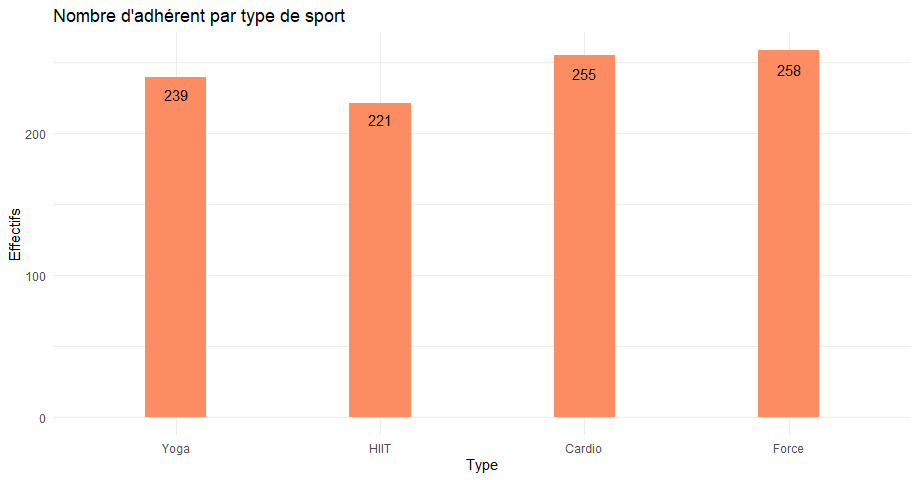
\includegraphics[width=\textwidth]{barplot_gym2.png}
		\end{subfigure}~
		\begin{subfigure}{0.48\textwidth}
		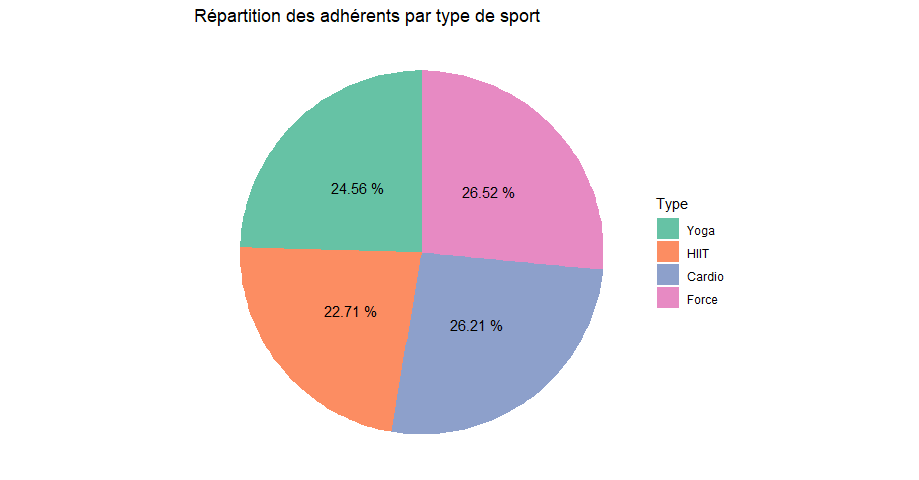
\includegraphics[width=\textwidth]{piechart_gym1.png}
		\end{subfigure}
		\end{figure}			
	\end{exampleblock}
\end{frame}

%------------------------------------------------
%	NEW SLIDE
%------------------------------------------------
\begin{frame}
	\begin{exampleblock}{\textbf{Remarque}}
		\begin{itemize}
		\item Pour une variable qualitative ordinale, on n'utilisera que des diagrammes en barres, afin de pas perdre le caractère ordonné de la variable.
		\item Supposons par exemple que l'on ait classé nos 973 adhérents par niveau de 1 \emph{(Débutant)} à 4 \emph{(Confirmé)}.
			\begin{center}
			\begin{tabular}{ccccc}
			Niveau & 1 & 2 & 3 & 4 \\
			\hline
			Effectif & 392 & 281 & 165 & 135
			\end{tabular}
			\end{center}
			
			\begin{center}
			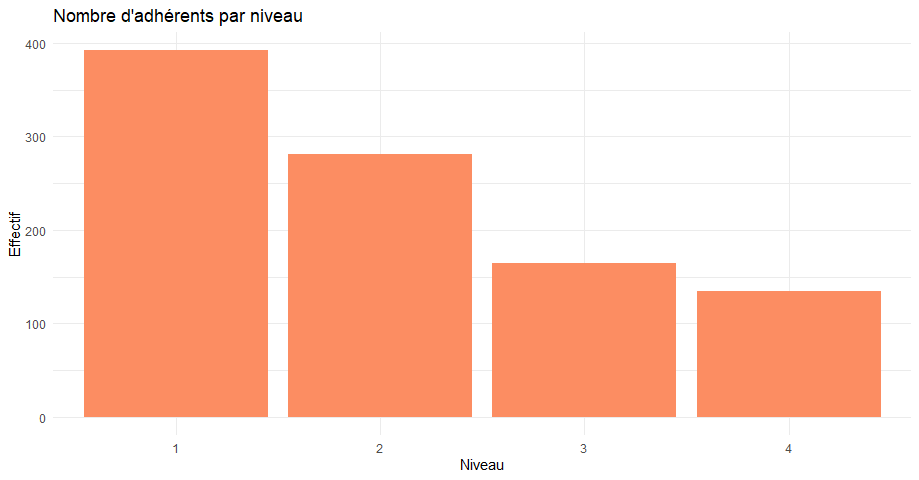
\includegraphics[scale=0.28]{barplot_gym3.png}
			\end{center}
		\end{itemize}
	\end{exampleblock}
\end{frame}

%~~~~~~~~~~~~~~~~~~~~~~~~~~~~~~~~~~~~~~~~~~~~~~~~
\section{Variables quantitatives}
%~~~~~~~~~~~~~~~~~~~~~~~~~~~~~~~~~~~~~~~~~~~~~~~~

%------------------------------------------------
%	NEW SLIDE
%------------------------------------------------
\begin{frame}[plain]

\vfill

\begin{center}
{\huge \textcolor{nyubluedark}{\textbf{3. Variables quantitatives}}}
\end{center}

\vfill

\end{frame}

%------------------------------------------------
%	NEW SLIDE
%------------------------------------------------
\begin{frame}
	\begin{block}{\textbf{Représentation graphique}}
		\begin{itemize}
		\item Lorsque la variable est \textbf{discrète} \emph{(et avec peu de modalités)}, on peut procéder comme si c'était une variable qualitative ordinale.
		\item Lorsque la variable est \textbf{continue}, on peut la représenter :
			\begin{itemize}
			\item par un \textbf{histogramme};
			\item  par un \textbf{boxplot} \emph{(boîte à moustaches)}.
			\end{itemize}
		\end{itemize}
	\end{block}
\end{frame}

%------------------------------------------------
%	NEW SLIDE
%------------------------------------------------
\begin{frame}
	\begin{block}{\textbf{Histogramme}}
		\begin{itemize}
		\item Un histogramme est un graphique à barres verticales accolées, obtenu après découpage en classes des observations.
		\item La surface de chaque barre est proportionnelle à l'effectif de la classe.
		\end{itemize}
	\end{block}
	
	\begin{exampleblock}{\textbf{Exemple}}
On a représenté ci-dessous un histogramme représentant la variable \og Temps hebdomadaire passé à la salle de sport \fg{} des individus observés.
		\begin{center}
		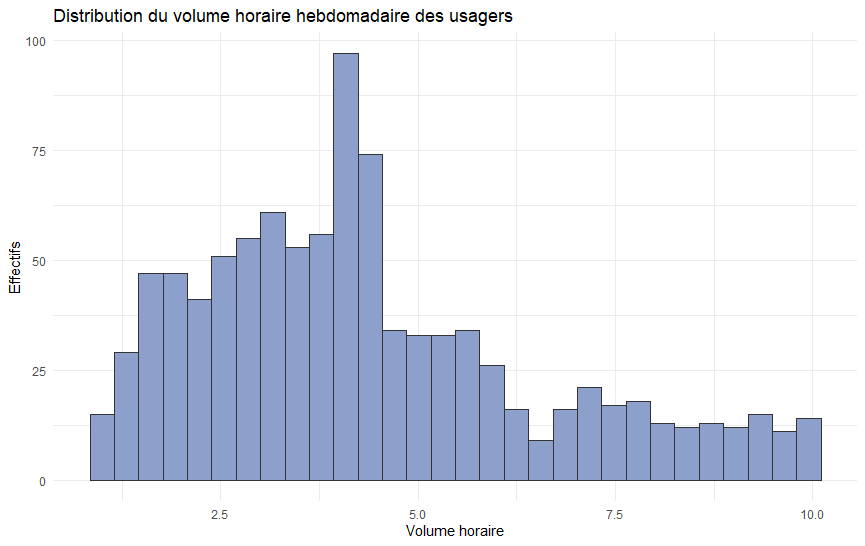
\includegraphics[scale=0.25]{histo_gym2.png} 
		\end{center}
	\end{exampleblock}
\end{frame}

%------------------------------------------------
%	NEW SLIDE
%------------------------------------------------
\begin{frame}

	\begin{exampleblock}{\textbf{Remarque}}
{\footnotesize 	Choisir un trop grand nombre $k$ de classe \og brouille \fg{} l'information.}
		\begin{figure}
		\centering
			\begin{subfigure}{0.4\textwidth}
			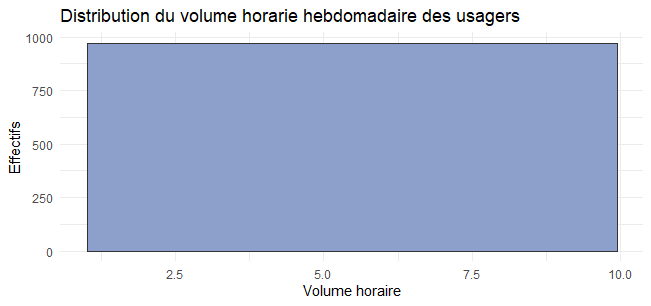
\includegraphics[width=\textwidth]{histo_gym_rk1.png}
			\caption{{\tiny $k=1$}}
			\end{subfigure}~
			\begin{subfigure}{0.4\textwidth}
			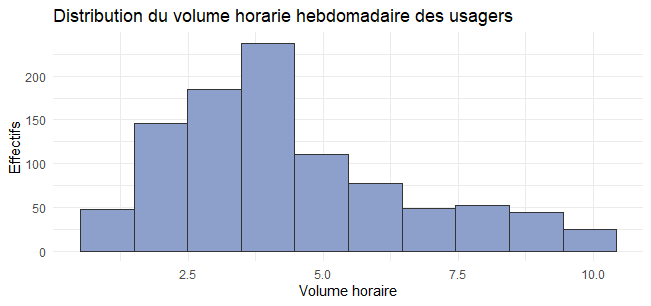
\includegraphics[width=\textwidth]{histo_gym_rk2.png}
			\caption{{\tiny $k=10$}}			
			\end{subfigure}
			
			\begin{subfigure}{0.4\textwidth}
			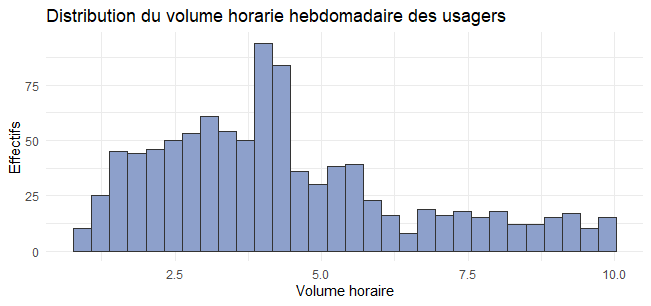
\includegraphics[width=\textwidth]{histo_gym_rk3.png}
			\caption{{\tiny $k=30$}}			
			\end{subfigure}~
			\begin{subfigure}{0.4\textwidth}
			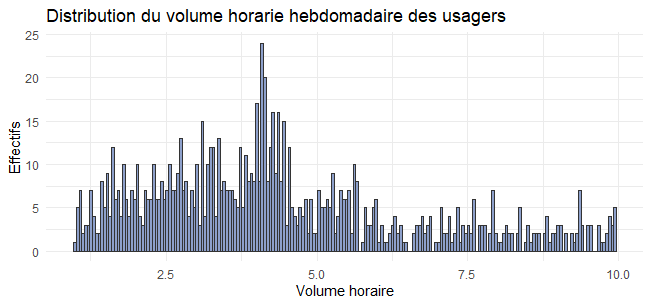
\includegraphics[width=\textwidth]{histo_gym_rk4.png}
			\caption{{\tiny $k=200$}}			
			\end{subfigure}
		\end{figure}
	\end{exampleblock}
\end{frame}

%------------------------------------------------
%	NEW SLIDE
%------------------------------------------------
\begin{frame}
	\begin{exampleblock}{\textbf{Remarque (suite)}}
	La difficulté est de déterminer le nombre $k$ de classes. Parmi les solutions courantes, on peut utiliser :
		\begin{itemize}
		\item La \textbf{formule de Sturges} :
			\[k=1+3.3 \log_{10}(n)\]
		où $n$ est l'effectif total de l'échantillon.
		\item La \textbf{formule de Yule} :
			\[k = 2.5 \times n^{1/4}.\]
		\end{itemize}			
	\end{exampleblock}
\end{frame}

%------------------------------------------------
%	NEW SLIDE
%------------------------------------------------
\begin{frame}
	\begin{block}{\textbf{Boxplot}}
		\begin{itemize}
		\item Il s'agit une représentation synthétique efficace des principaux indicateurs statistiques d'une variable quantitative.
		\item Un tel diagramme fournit des indicateurs de position et de dispersion de la variable considérée.
		\end{itemize}
	\end{block}
\end{frame}

\begin{frame}
	\begin{exampleblock}{\textbf{Exemple}}
	\begin{footnotesize}
	 Si on s'intéresse au temps hebdomadaire passé par les usagers à la salle de sport, le langage \textsf{R} représente ainsi :
			\begin{itemize}
			\item une boîte délimitée par les quartiles $Q_1$ et $Q_3$;
			\item une ligne à l'intérieur de cette boîte indiquant la médiane;
			\item des \og moustaches \fg{} s'étendant de part et d'autre jusqu'à la dernière valeur éloignée de moins de $1.5(Q_3-Q_1)$.
			\item Les valeurs en-dehors de ces \og moustaches \fg{} sont des \textbf{outliers}.
			\end{itemize}
	\end{footnotesize}
		\begin{center}
		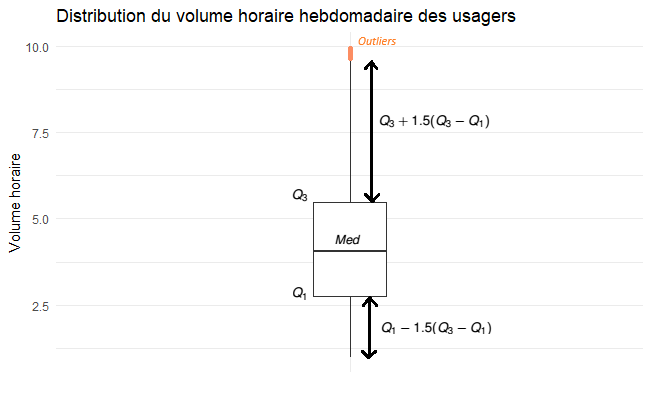
\includegraphics[scale=0.35]{box_plot_explain.png}
		\end{center}
	\end{exampleblock}

\end{frame}

%~~~~~~~~~~~~~~~~~~~~~~~~~~~~~~~~~~~~~~~~~~~~~~~~
\section{Indicateurs statistiques}
%~~~~~~~~~~~~~~~~~~~~~~~~~~~~~~~~~~~~~~~~~~~~~~~~

%------------------------------------------------
%	NEW SLIDE
%------------------------------------------------
\begin{frame}[plain]

\vfill

\begin{center}
{\huge \textcolor{nyubluedark}{\textbf{4. Indicateurs statistiques}}}
\end{center}

\vfill

\end{frame}

%------------------------------------------------
%	NEW SLIDE
%------------------------------------------------
\begin{frame}

\vfill

\textcolor{nyubluedarker}{\faCogs} On considère dans cette section des \textbf{variables quantitatives}.

\vspace*{1cm}

\textcolor{nyubluedarker}{\faCogs} Les indicateurs statistiques que l'on calcule pour de telles variables sont de deux ordres :
	\begin{itemize}
	\item indicateurs de position \emph{(Moyenne,Médiane,Quartiles,...)};
	\item indicateurs de dispersion \emph{(Ecart inter-quartiles, Variance...)}.
	\end{itemize}

\vspace*{1cm}

\textcolor{nyubluedarker}{\faLightbulb[regular]} On ne peut décrire efficacement un jeu de données qu'en associant ces deux types d'indicateurs, mais ce n'est pas toujours suffisant...

\vfill
\end{frame}

%~~~~~~~~~~~~~~~~~~~~~~~~~~~~~~~~~~~~~~~~~~~~~~~~
\subsection{Indicateurs de position}
%~~~~~~~~~~~~~~~~~~~~~~~~~~~~~~~~~~~~~~~~~~~~~~~~

%------------------------------------------------
%	NEW SLIDE
%------------------------------------------------
\begin{frame}[plain]

\vfill

\begin{center}
{\huge \textcolor{nyubluedark}{\textbf{4.1. Indicateurs de position}}}
\end{center}

\vfill

\end{frame}

%------------------------------------------------
%	NEW SLIDE
%------------------------------------------------
\begin{frame}
	\begin{block}{\textbf{Moyenne arithmétique}}
	Si on considère un échantillon de valeurs $(x_i)_{1\leqslant i \leqslant n}$, alors la moyenne de ces valeurs est
		\[
		\overline{x} = \dfrac{1}{n} \sum_{i=1}^n x_i
		\]
	\end{block}
	
	\begin{exampleblock}{\textbf{Avantages / Inconvénients}}
		\begin{itemize}
		\item[\faPlusCircle] La moyenne arithmétique minimise la somme des carrés des écarts à une valeur $A$, i.e.
			\[
			\overline{x} = \underset{A \in \R}{\argmin} \ \sum_{i=1}^n (x_i-A)^2.
			\]
		\item[\faMinusCircle] Elle est très sensible aux valeurs extrêmes...
		\end{itemize}
	\end{exampleblock}
	
\end{frame}

%------------------------------------------------
%	NEW SLIDE
%------------------------------------------------
\begin{frame}
	\begin{exampleblock}{\textbf{Exemple}}
		\begin{itemize}
		\item Si on considère 100 salariés d'une entreprise qui gagnent entre 2000\euro \ et 4000\euro \ bruts, on aura une moyenne comprise entre 2000 et 4000 euros brut.
		\item Supposons qu'on ajoute le salaire du chef d'entreprise, qui est de 1 000 000\euro \ bruts !
		
		La moyenne des salaires sera alors comprise entre 11 881.18 et 13 861.39 euros brut, soit une augmentation d'environ 10 000\euro \ !!!
		\end{itemize}

	\end{exampleblock}
\end{frame}

%------------------------------------------------
%	NEW SLIDE
%------------------------------------------------
\begin{frame}
	\begin{block}{\textbf{Médiane}}
		\begin{itemize}
		\item Il s'agit d'une valeur $\widetilde{x}$ permettant de scinder un jeu de données $(x_i)_{1\leqslant i \leqslant n}$ en deux groupes de même effectif.
		\item Au moins la moitié des valeurs $x_i$ sont \textbf{inférieures} ou égales à $\widetilde{x}$...
		\item ... et au moins la moitié des valeurs $x_i$ sont \textbf{supérieures} ou égales à $\widetilde{x}$.
		\end{itemize}
	\end{block}
	
	\medskip
	
\textcolor{nyupurple}{\faCogs} Si $n$ est impair, on prend la valeur centrale de la série statistique, soit la $\frac{n+1}{2}$-ème valeur.

\textcolor{nyupurple}{\faCogs} Si $n$ est pair, on prend la moyenne de la $n$-ème et de la $n+1$-ème valeur.

\end{frame}

%------------------------------------------------
%	NEW SLIDE
%------------------------------------------------
\begin{frame}
	\begin{exampleblock}{\textbf{Exemple}}
	Reprenons les données de salaire d'une entreprise (100 salariés + chef d'entreprise).
		\begin{center}
		\begin{tabular}{ccccccc}
		\hline
		Salaire brut (\euro) & 2000 & 2500 & 3000 & 3500 & 4000 & 1 000 000 \\
		Effectifs & 50 & 20 & 15 & 10 & 5 & 1 \\
		\hline
		\end{tabular}
		\end{center}
		\begin{itemize}
		\item Sans le chef d'entreprise, le salaire médian est de 2250\euro \ bruts.
		\item Avec le chef d'entreprise, le salaire médian est de  2500\euro \ bruts.
		\end{itemize}
	\end{exampleblock}
\end{frame}

%------------------------------------------------
%	NEW SLIDE
%------------------------------------------------
\begin{frame}
	\begin{exampleblock}{\textbf{Avantages / Inconvénients}}
		\begin{itemize}
		\item[\faPlusCircle] La médiane minimise la somme des valeurs absolues des écarts à une valeur $A$, i.e.
			\[
			\widetilde{x} = \underset{A \in \R}{\argmin} \ \sum_{i=1}^n \left| x_i-A\right|.
			\]
		\item[\faPlusCircle] La médiane est peu sensible aux valeurs extrêmes.
		\item[\faMinusCircle] Elle ne tient pas compte des valeurs de la série statistique, mais de leur rang : elle est donc plus sensible aux fluctuations d'échantillon que la moyenne.
		\item[\faMinusCircle] Peu pratique à calculer.
		\end{itemize}
	\end{exampleblock}
\end{frame}

%------------------------------------------------
%	NEW SLIDE
%------------------------------------------------
\begin{frame}
	\begin{exampleblock}{\textbf{Remarque}}
		\begin{itemize}
		\item Les indicateurs de moyenne et médiane peuvent ne pas suffire pour résumer une série statistique, ou effectuer des comparaisons.
		\item On a représenté ci-dessous les histogrammes de deux séries statistiques.
			\begin{center}
			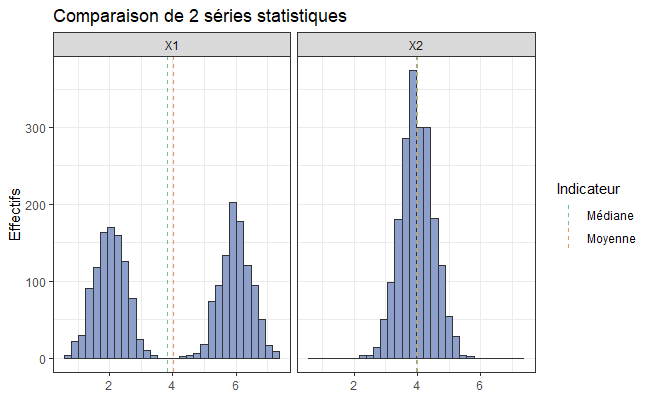
\includegraphics[scale=0.5]{comp_moy_med.png}
			\end{center}
		\end{itemize}

	\end{exampleblock}
\end{frame}

%------------------------------------------------
%	NEW SLIDE
%------------------------------------------------
\begin{frame}
	\begin{block}{\textbf{Mode}}
\begin{footnotesize}
		\begin{itemize}
		\item On appelle \textbf{mode} d'une série statistique la valeur ayant le plus grand effectif.
		\item Si on regroupe la série en classes, la \textbf{classe modale} est la classe ayant le plus grand effectif.
		\end{itemize}
\end{footnotesize}
	\end{block}
	
	\begin{exampleblock}{\textbf{Exemple}}
{\footnotesize 	Dans l'exemple précédent, on peut distinguer deux modes sur la première série, contre un seul dans la seconde.}
		\begin{center}
		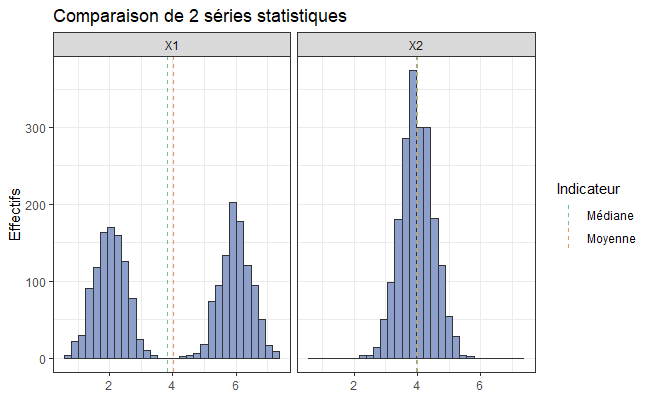
\includegraphics[scale=0.35]{comp_moy_med.png}
		\end{center}
	\end{exampleblock}
\end{frame}

%------------------------------------------------
%	NEW SLIDE
%------------------------------------------------
\begin{frame}
	\begin{block}{\textbf{Quantiles}}
		\begin{itemize}
		\item Le \textbf{quantile} d'ordre $p$ d'une série statistique est la plus petite valeur $q$ de la série telle qu'une proportion $p$ des valeurs sont inférieur ou égale à $q$.
		\item On distingue en particulier :
			\begin{itemize}
			\item les \textbf{quartiles} $Q_1$ et $Q_3$ \emph{(quantiles d'ordres 0.25 et 0.75)};
			\item les \textbf{déciles} $D_1,D_2,\ldots,D_9$ \emph{(quantiles d'ordres $0.1,0.2,\ldots,0.9$)}.
			\end{itemize}
		\end{itemize}
	\end{block}
\end{frame}

%------------------------------------------------
%	NEW SLIDE
%------------------------------------------------
\begin{frame}
	\begin{exampleblock}{\textbf{Exemple}}
	\begin{itemize}
	\item Reprenons l'exemple des salaires.
		\begin{center}
			\begin{tabular}{ccccccc}
			\hline
			Salaire brut (\euro) & 2000 & 2500 & 3000 & 3500 & 4000 & 1 000 000 \\
			Effectifs & 50 & 20 & 15 & 10 & 5 & 1 \\
			\hline
			\end{tabular}
		\end{center}
	\item On a
		\begin{itemize}
		\item $Q_1 = 2000$ et $Q_3=3000$;
		\item $D_1 = 2000$ et $D_9=3500$.
		\end{itemize}
	\end{itemize}
	\end{exampleblock}
\end{frame}

%~~~~~~~~~~~~~~~~~~~~~~~~~~~~~~~~~~~~~~~~~~~~~~~~
\subsection{Indicateurs de dispersion}
%~~~~~~~~~~~~~~~~~~~~~~~~~~~~~~~~~~~~~~~~~~~~~~~~

%------------------------------------------------
%	NEW SLIDE
%------------------------------------------------
\begin{frame}[plain]

\vfill

\begin{center}
{\huge \textcolor{nyubluedark}{\textbf{4.2. Indicateurs de dispersion}}}
\end{center}

\vfill

\end{frame}

%------------------------------------------------
%	NEW SLIDE
%------------------------------------------------
\begin{frame}

\textcolor{nyupurple}{\faLightbulb[regular]} Un indice de dispersion  permet de mesurer l'écartement des valeurs les unes par rapport aux autres, ou bien par rapport à un indice de position.
	
	\begin{block}{\textbf{Etendue}}
	L'étendue d'une série statistique $(x_i)_{1\leqslant i \leqslant n}$ est donnée par
		\[
		E(x) = \underset{1 \leqslant i \leqslant n}{\max} \ x_i - \underset{1 \leqslant i \leqslant n}{\min} \ x_i.
		\]
	\end{block}
	
	\begin{block}{\textbf{Ecarts inter-quantiles}}
	On peut considérer
		\begin{itemize}
		\item l'écart inter-quartiles : $Q_3-Q_1$;
		\item l'écart inter-déciles : $D_9-D_1$.
		\end{itemize}
	\end{block}
\end{frame}

%------------------------------------------------
%	NEW SLIDE
%------------------------------------------------
\begin{frame}
	\begin{block}{\textbf{Variance et écart-type}}
		\begin{itemize}
		\item La \textbf{variance} d'une série correspond $(x_i)_{1\leqslant i \leqslant n}$ à la moyenne des carrés des écarts à la moyenne :
			\[
			V(x) = \dfrac{1}{n}\sum_{i=1}^n \left( x_i - \overline{x}\right)^2.
			\]
		\item L'\textbf{écart-type} est la racine carrée de la variance :
			\[
			\sigma(x) = \sqrt{V(x)}.
			\]
		\item Plus ces indices sont grands, plus les valeurs de la série sont dispersées autour de la moyenne.
		\end{itemize}
	\end{block}
	
	\begin{exampleblock}{\textbf{Avantages / Inconvénients}}
		\begin{itemize}
		\item[\faPlusCircle] Faciles à calculer.
		\item[\faMinusCircle] Sensibles aux valeurs extrêmes...
		\end{itemize}
	\end{exampleblock}
\end{frame}

%------------------------------------------------
%	NEW SLIDE
%------------------------------------------------
\begin{frame}
	\begin{block}{\textbf{MAD}}
	Le \textbf{MAD} d'une série $(x_i)_{1 \leqslant i \leqslant n}$ correspond à la médiane des écarts absolus à la médiane :
		\[
		MAD (x) = Med \left( \left| x_i - \widetilde{x} \right| \right)_{1 \leqslant i \leqslant n}.
		\]
	\end{block}
	
	\begin{exampleblock}{\textbf{Avantages / Inconvénients}}
		\begin{itemize}
		\item[\faPlusCircle] Peu sensible aux valeurs extrêmes.
		\item[\faMinusCircle] Peu pratique à calculer.
		\end{itemize}
	\end{exampleblock}
\end{frame}

%------------------------------------------------
%	NEW SLIDE
%------------------------------------------------
\begin{frame}
	\begin{block}{\textbf{Valeurs atypiques}}
	Plusieurs critères permettent de considérer certaines valeurs d'une série $(x_i)_{1 \leqslant i \leqslant n}$ comme atypiques \emph{(\textbf{outliers})}.
	
	On considère souvent une valeur $x_i$ comme atypique si :
		\begin{itemize}
		\item $x_i > Q_3 + 1.5(Q_3-Q_1)$ ou $x_i<Q_1 - 1.5(Q_3-Q_1)$;
		\item ou bien $\left| x_i - \overline{x} \right| > 3 \sigma(x)$;
		\item ou bien $\left| x_i - \widetilde{x} \right| > 4.45 \times MAD(x)$.
		\end{itemize}
	\end{block}
\end{frame}

%------------------------------------------------
%	NEW SLIDE
%------------------------------------------------
\begin{frame}[fragile]
	\begin{exampleblock}{\textbf{Exemple}}
		\begin{itemize}
		\item On considère à nouveau les 973 clients de la salle de sport interrogés sur leur volume d'entraînement hebdomadaire \emph{(en heures)}.
		\item On a calculé différents indicateurs statistiques de cette série, nommée \texttt{Vol}, avec \textsf{R} :
\begin{minted}[bgcolor=nyupurple!10,fontsize=\scriptsize]{R}
# Moyenne
mean(Vol)
# Médiane
median(Vol)
# Quartiles Q1 et Q3
quantile(Vol,probs = c(0.25,0.75))
# MAD
mad(Vol,constant = 1)
# Variance et Ecart-type
var(Vol)*972/973
sd(Vol)*sqrt(972/973)
\end{minted}
		\end{itemize}
	\end{exampleblock}
\end{frame}

%------------------------------------------------
%	NEW SLIDE
%------------------------------------------------
\begin{frame}
	\begin{exampleblock}{\textbf{Exemple (suite)}}
	\begin{itemize}
	\item On obtient alors
		\begin{multicols}{3}
		\begin{itemize}
		\item $\overline{x} = 4.374985$
		\item $\widetilde{x} = 4.05$
		\item $Q_1 = 2.76; \ Q_3=5.48$
		\item $MAD(x) = 1.35$
		\item $V(x) = 4.739766$
		\item $\sigma(x) = 2.1771$
		\end{itemize}
	\end{multicols}
	\item Un individu peut donc être considéré comme un outlier si son volume horaire d'entraînement :
		\begin{itemize}
		\item n'appartient pas à l'intervalle $[-1.32 ; 9.56]$ \emph{(critère inter-quartiles)};
		\item n'appartient pas à l'intervalle $[-1.9575 ; 10.0575]$ \emph{(critère MAD)};
		\item n'appartient pas à l'intervalle $[-2.1529 ; 10.90293]$ \emph{(critère écart-type)}.
		\end{itemize}
	\end{itemize}
	\end{exampleblock}
\end{frame}

%~~~~~~~~~~~~~~~~~~~~~~~~~~~~~~~~~~~~~~~~~~~~~~~~
\section{Lien entre deux variables}
%~~~~~~~~~~~~~~~~~~~~~~~~~~~~~~~~~~~~~~~~~~~~~~~~

%------------------------------------------------
%	NEW SLIDE
%------------------------------------------------
\begin{frame}[plain]

\vfill

\begin{center}
{\huge \textcolor{nyubluedark}{\textbf{5. Lien entre deux variables}}}
\end{center}

\vfill

\end{frame}

%~~~~~~~~~~~~~~~~~~~~~~~~~~~~~~~~~~~~~~~~~~~~~~~~
\subsection{Lien entre deux variables quantitatives}
%~~~~~~~~~~~~~~~~~~~~~~~~~~~~~~~~~~~~~~~~~~~~~~~~

%------------------------------------------------
%	NEW SLIDE
%------------------------------------------------
\begin{frame}[plain]

\vfill

\begin{center}
{\huge \textcolor{nyubluedark}{\textbf{5.1 Lien entre deux variables quantitatives}}}
\end{center}

\vfill

\end{frame}

%------------------------------------------------
%	NEW SLIDE
%------------------------------------------------
\begin{frame}
\textcolor{nyubluedarker}{\faCogs} Considérons deux séries $(x_i)_{1 \leqslant i \leqslant n}$ et $(y_i)_{1 \leqslant i \leqslant n}$ correspondant à deux variables quantitatives observées dans un échantillon de taille $n$.

\medskip

\textcolor{nyubluedarker}{\faLightbulb[regular]} On peut représenter graphiquement un potentiel lien entre les deux variables par un \textbf{nuage de points}.

	\begin{center}
	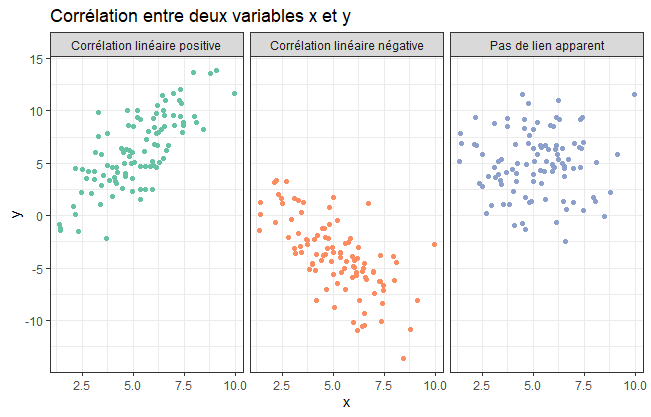
\includegraphics[scale=0.45]{expl_cor.png}
	\end{center}
\end{frame}

%------------------------------------------------
%	NEW SLIDE
%------------------------------------------------
\begin{frame}
	\begin{block}{\textbf{Définitions}}
		\begin{itemize}
		\item La \textbf{covariance} empirique des séries $x$ et $y$ est donnée par
			\[
			Cov(x,y) = \dfrac{1}{n}\sum_{i=1}^n \left(x_i - \overline{x} \right) \left(y_i - \overline{y} \right).
			\]
		\item Le coefficient de \textbf{corrélation} empirique \emph{(de Pearson)} est alors
			\[
			\rho (x,y) = \dfrac{Cov(x,y)}{\sigma (x) \sigma (y)}.
			\]
		\end{itemize}
	\end{block}
	
	\begin{exampleblock}{\textbf{Remarque}}
	On a en particulier $Cov(x,x) = V(x)$ et $\rho(x,x)$ = 1.
	\end{exampleblock}
\end{frame}

%------------------------------------------------
%	NEW SLIDE
%------------------------------------------------
\begin{frame}
	\begin{alertblock}{\textbf{Propriétés}}
		\begin{itemize}
		\item On a $Cov(x,y) =Cov(y,x)$ et $\rho(x,y) = \rho(y,x)$.
		\item On a $-1 \leqslant \rho(x,y) \leqslant 1$.
		\item On a $ \left| \rho(x,y) \right| = 1$ \underline{ssi} il existe deux réels $a$ et $b$ tels que
		\[y_i=ax_i+b, \ \forall i \in \{1,\ldots,n\}.\]
		\item Le coefficient de corrélation est invariant par transformation linéaire \emph{(changement d'échelle)}, i.e. si 
			\[
			\forall i \in \{1,\ldots n\}, \ \widetilde{x}_i=\alpha x_i + \beta,
			\]
		alors $\rho(\widetilde{x},y) = \rho(x,y)$.
		\end{itemize}
	\end{alertblock}
\end{frame}

%------------------------------------------------
%	NEW SLIDE
%------------------------------------------------
\begin{frame}
	\begin{exampleblock}{\textbf{Exemple}}
{\footnotesize 	Le jeu de données \texttt{airquality} disponible sur \textsf{R} est constitué des mesures d'ozone, de radiation solaire, de vent et de température prises pendant 153 jours.}
\begin{footnotesize}
		\begin{center}
		\begin{tabular}{rrrrr}
  			\hline
 		& Ozone & Solar.R & Wind & Temp \\[-3pt] 
  		\hline
		1 &  41 & 190 & 7.40 &  67 \\[-3pt]  
  		2 &  36 & 118 & 8.00 &  72 \\[-3pt]  
  		3 &  12 & 149 & 12.60 &  74 \\[-3pt]  
  		4 &  18 & 313 & 11.50 &  62 \\[-3pt]  
   		\hline
		\end{tabular}
		\end{center}
		
		\begin{center}
		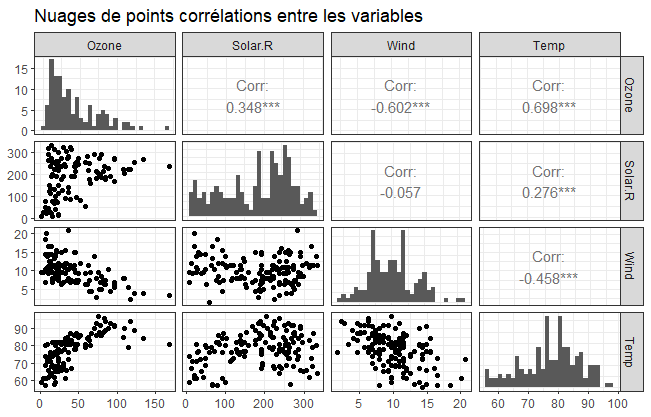
\includegraphics[scale=0.3]{cor_air_quality.png}
		\end{center}
\end{footnotesize}
	\end{exampleblock}
\end{frame}

%------------------------------------------------
%	NEW SLIDE
%------------------------------------------------
\begin{frame}
	\begin{exampleblock}{\textbf{Exemple (suite)}}
	\begin{footnotesize}
	On peut écrire la \textbf{matrice de corrélation} :
			\[
			M = \begin{pmatrix}
			1 & 0.348 & -0.602 & 0.698 \\
			0.348 & 1 & -0.057 & 0.276 \\
			-0.602 & -0.057 & 1 & -0.458 \\
			0.698 & 0.276 & -0.458 & 1
			\end{pmatrix}.
			\]
		\begin{figure}
		\centering
		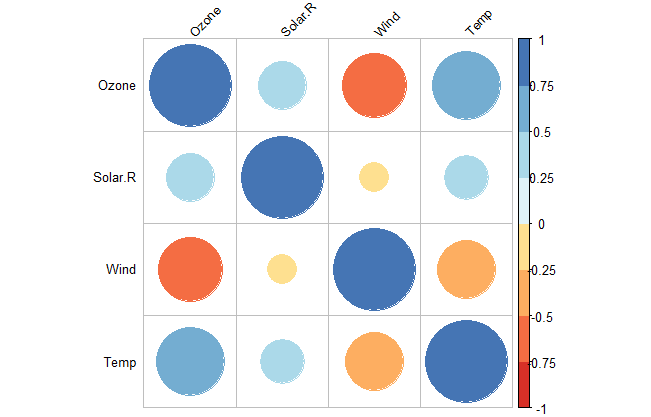
\includegraphics[scale=0.35]{corrplot.png}
		\end{figure}
	\end{footnotesize}
	\end{exampleblock}
\end{frame}

%~~~~~~~~~~~~~~~~~~~~~~~~~~~~~~~~~~~~~~~~~~~~~~~~
\subsection{Lien entre une variable qualitative et une variables quantitative}
%~~~~~~~~~~~~~~~~~~~~~~~~~~~~~~~~~~~~~~~~~~~~~~~~

%------------------------------------------------
%	NEW SLIDE
%------------------------------------------------
\begin{frame}[plain]

\vfill

\begin{center}
{\huge \textcolor{nyubluedark}{\textbf{5.2 Lien entre une variable qualitative et une variable quantitative}}}
\end{center}

\vfill

\end{frame}

%------------------------------------------------
%	NEW SLIDE
%------------------------------------------------
\begin{frame}

\vfill

\textcolor{nyubluedarker}{\faCogs} On considère une variable $x$ qualitative prenant $K$ modalité, et une variable quantitative $y$ de moyenne $\overline{y}$ et de variance $V(y)$, dans un échantillon de taille $n$.

\medskip

\textcolor{nyubluedarker}{\faCogs} Pour chaque modalité $k \in \{1,\ldots , K\}$, on note :
	\begin{itemize}
	\item $n_k$ l'effectif de la modalité $k$;
	\item $\overline{y}_k$ la moyenne de la variable $y$ pour les individus appartenant au groupe $k$;
	\item $V_k(y)$ la variance de la variable $y$ pour les individus appartenant au groupe $k$.
	\end{itemize}	
	
	\begin{center}
	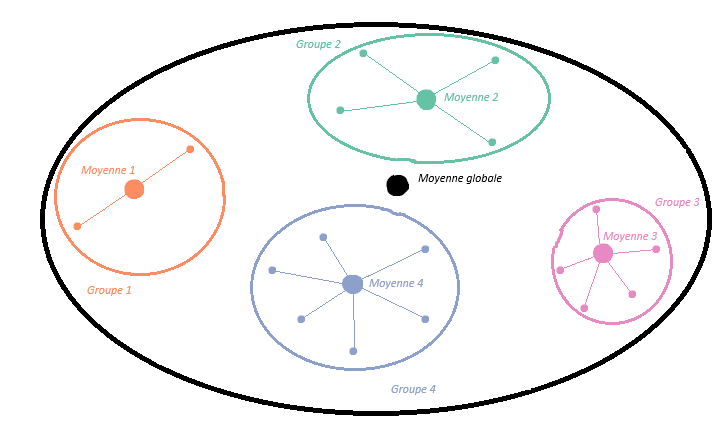
\includegraphics[scale=0.4]{pres_var.png}
	\end{center}
	
	\vfill
	
\end{frame}

%------------------------------------------------
%	NEW SLIDE
%------------------------------------------------
\begin{frame}
	\begin{exampleblock}{\textbf{Exemple}}
\begin{footnotesize}
	Considérons le jeu de donnée \texttt{iris} dans \textsf{R}, contenant 150 observations de fleurs.
		\begin{center}
\begin{tabular}{rrrrrl}
  \hline
 Obs & Sepal.Length & Sepal.Width & Petal.Length & Petal.Width & Species \\[-3pt]
  \hline
1 & 5.10 & 3.50 & 1.40 & 0.20 & setosa \\[-3pt] 
  2 & 4.90 & 3.00 & 1.40 & 0.20 & setosa \\[-3pt] 
  51 & 7.00 & 3.20 & 4.70 & 1.40 & versicolor \\[-3pt] 
  107 & 4.90 & 2.50 & 4.50 & 1.70 & virginica \\[-3pt] 
   \hline
\end{tabular}
		\end{center}
	On peut représenter la distribution de la variable \texttt{Petal.Length} en fonction de l'espèce sur un même graphique.
\end{footnotesize}
		\begin{figure}
		\centering
		\begin{subfigure}{0.3\textwidth}
		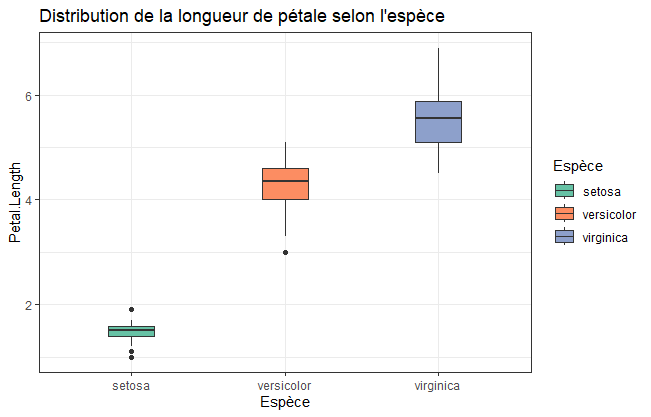
\includegraphics[width=\textwidth]{boxplot_iris.png}
		\end{subfigure}~
		\begin{subfigure}{0.3\textwidth}
		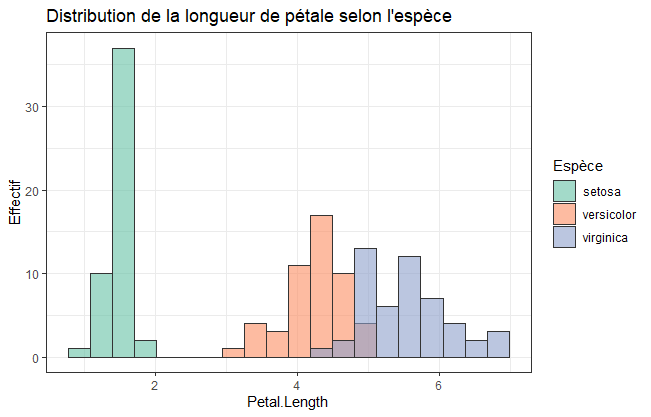
\includegraphics[width=\textwidth]{histo_iris.png}
		\end{subfigure}
		\end{figure}
	\end{exampleblock}
\end{frame}

%------------------------------------------------
%	NEW SLIDE
%------------------------------------------------
\begin{frame}
	
	\begin{block}{\textbf{Définitions}}
\begin{small}
		\begin{itemize}
		\item On appelle \textbf{variance inter-groupes}
			\[
			V_{inter} = \dfrac{1}{n} \sum_{k=1}^K n_k \left( \overline{y}_k - \overline{y}\right)^2.
			\]
		\item On appelle \textbf{variance intra-groupes}
			\[
			V_{intra} = \dfrac{1}{n} \sum_{k=1}^K n_k V_k(y).
			\]
		\end{itemize}
\end{small}
	\end{block}

	\begin{alertblock}{\textbf{Décomposition de la variance}}
\begin{small}
	On a la formule de K\"onig-Huygens
		\[
		V(y) = V_{intra} + V_{inter}.
		\]
\end{small}
	\end{alertblock}
\end{frame}

%------------------------------------------------
%	NEW SLIDE
%------------------------------------------------
\begin{frame}
\textcolor{nyupurple}{\faLightbulb[regular] \ \textbf{Schéma :}} $V(y) = V_{intra} + V_{inter}$.

	\begin{figure}
	\centering
	\begin{subfigure}{0.45\textwidth}
	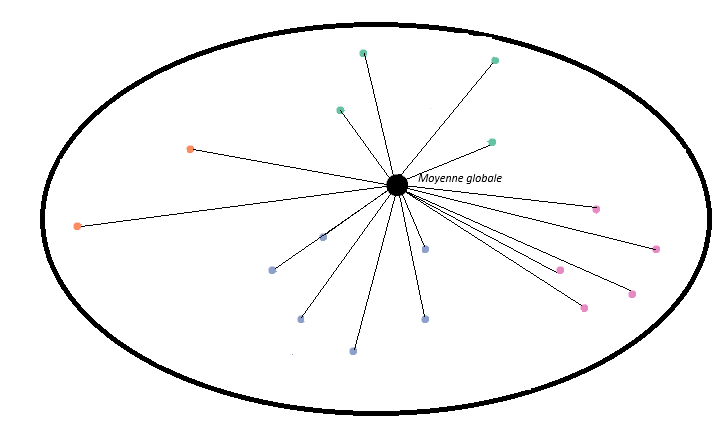
\includegraphics[width=\textwidth]{var_globale.png}
	\end{subfigure}~
	\begin{subfigure}{0.45\textwidth}
	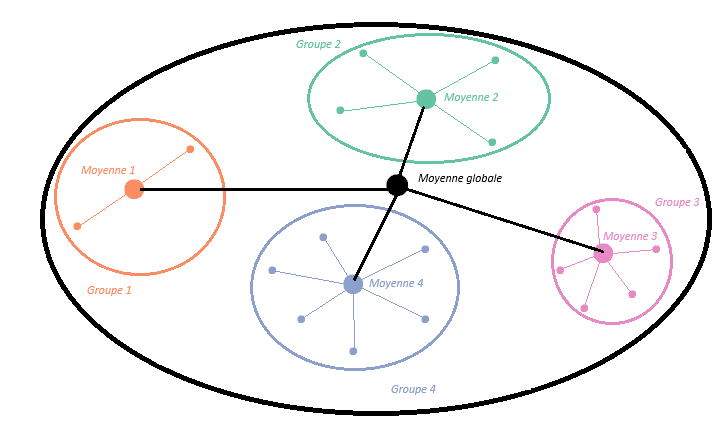
\includegraphics[width=\textwidth]{decomp_var.png}
	\end{subfigure}
	\end{figure}
	
	\begin{block}{\textbf{Variance expliquée}}
	La proportion de variance de $y$ expliquée par la variable $x$ est $\dfrac{V_{inter}}{V(y)}$.
	\end{block}
\end{frame}

%------------------------------------------------
%	NEW SLIDE
%------------------------------------------------
\begin{frame}
	\begin{exampleblock}{\textbf{Exemple}}
		\begin{footnotesize}
		\begin{itemize}
		\item Toujours avec le jeu de données \texttt{iris} dans \textsf{R}, on a pour la variable $y=$ \texttt{Petal.Length} :
			\[
			\overline{y} = 3.758, \quad \overline{y}_{setosa} = 1.462, \quad \overline{y}_{versicolor}=4.260, \quad \overline{y}_{virginica} = 5.552
			\]
			et
			\[
			V(y) = 3.096, \quad V_{setosa}(y) = 0.030, \quad V_{versicolor}(y)=0.219, \quad V_{virginica}(y) = 0.303.
			\]
		\item On calcule la variance intra-groupes :
			\[
			V_{intra} = \dfrac{1}{150} \times \left( 50 \times 0.03 + 50 \times 50\times 0.303 \right) = 0.184,
			\]
		et on en déduit la variance inter-groupes :
			\[
			V_{inter} = V(y) - V_{intra} = 2.912.
			\]
		\item La proportion de variance de \texttt{Petal.Length} expliquée par la variable \texttt{Espèce} est donc de :
			\[
			\dfrac{V_{inter}}{V(y)} \approx 0.941.
			\]
		\end{itemize}
		\end{footnotesize}
	\end{exampleblock}
\end{frame}

%~~~~~~~~~~~~~~~~~~~~~~~~~~~~~~~~~~~~~~~~~~~~~~~~
\subsection{Lien entre deux variables qualitatives}
%~~~~~~~~~~~~~~~~~~~~~~~~~~~~~~~~~~~~~~~~~~~~~~~~

%------------------------------------------------
%	NEW SLIDE
%------------------------------------------------
\begin{frame}[plain]

\vfill

\begin{center}
{\huge \textcolor{nyubluedark}{\textbf{5.3 Lien entre deux variables qualitatives}}}
\end{center}

\vfill

\end{frame}

%------------------------------------------------
%	NEW SLIDE
%------------------------------------------------
\begin{frame}
\begin{small}
\textcolor{nyubluedarker}{\faCogs} On considère deux variables qualitatives $x$ et $y$ prenant respectivement $J$ et $K$ modalités, pour un échantillon de taille $n$.

\textcolor{nyubluedarker}{\faLightbulb[regular]} On présente généralement ces données sous la forme d'une \textbf{table de contingence}.
\end{small}
	
	\begin{exampleblock}{\textbf{Exemple}}
	{\small Supposons que l'on ait mené une enquête auprès de 100 personnes sur leur boisson préférée, selon la tranche d'âge.}
\begin{scriptsize}
		\begin{center}
		\begin{tabular}{|c|c|c|c|c|}
		\hline
		\diagbox[height=0.5cm]{$x$ \ }{$y$} & Café & Thé & Jus de fruit & Total \\ \hline
		Jeunes & 5 & 15 & 20 & 40 \\ \hline
		Seniors & 20 & 25 & 15 & 60 \\ \hline
		Total & 25 & 40 & 35 & 100\\ \hline
		\end{tabular}
		\end{center}
		\begin{itemize}
		\item On a ici $J=2$ et $K=3$.
		\item Pour $1 \leqslant j \leqslant J$ et $1 \leqslant k \leqslant K$, on note :
			\begin{itemize}
			\item $n_{j,k}$ le nombre d'individus satisfaisant à la fois $x=j$ et $y=k$;
			\item $n_{j,\cdot}$ le nombre d'individus satisfaisant $x=j$ \emph{(effectif ligne $j$)};
			\item $n_{\cdot,k}$ le nombre d'individus satisfaisant $y=k$ \emph{(effectif colonne $k$)}.
			\end{itemize}
		\item Ici, $n_{2,1} = 20$, $n_{2,\cdot}=60$ et $n_{\cdot,1} =25$.
		\end{itemize}			

\end{scriptsize}
	\end{exampleblock}

\end{frame}

%------------------------------------------------
%	NEW SLIDE
%------------------------------------------------
\begin{frame}
\textcolor{nyubluedarker}{\faLightbulb[regular]} On peut représenter un tel tableau par un diagramme en barres :

	\begin{center}
	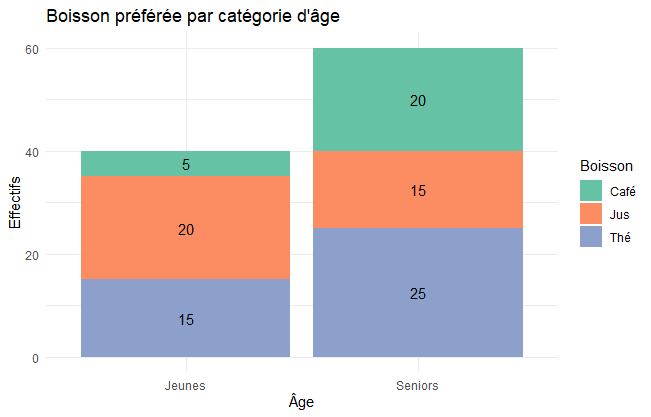
\includegraphics[scale=0.7]{lien_quali_raw.png}
	\end{center}
\end{frame}

%------------------------------------------------
%	NEW SLIDE
%------------------------------------------------
\begin{frame}
	\begin{block}{\textbf{Définition}}
		\begin{itemize}
		\item On appelle tableau des \textbf{profils-lignes} le tableau des fréquences conditionnelles $\dfrac{n_{j,k}}{n_{j,\cdot}}$ \emph{(chaque ligne somme à 1)};
		\item On appelle tableau des \textbf{profils-colonnes} le tableau des fréquences conditionnelles $\dfrac{n_{j,k}}{n_{\cdot,k}}$ \emph{(chaque colonne somme à 1)}.
		\end{itemize}
	\end{block}
	
	\begin{exampleblock}{\textbf{Exemple}}
	Dans l'exemple précédent, le tableau des profils-lignes est donné par
		\begin{center}
		\begin{scriptsize}
		\begin{tabular}{|c|c|c|c|}
		\hline
		 & Café & Thé & Jus de fruit \\
		\hline
		 & & & \\[-10pt]
		Jeunes & $\dfrac{5}{40} = 0.125$ & $\dfrac{15}{40} = 0.375$ & $\dfrac{20}{40} = 0.5$  \\[5pt] \hline
		 & & & \\[-10pt]
		Seniors & $\dfrac{20}{60} = 1/3 $ & $\dfrac{25}{60} = 5/12$ & $\dfrac{15}{60} = 1/4$ \\[5pt] \hline
		\end{tabular}
		\end{scriptsize}
		\end{center}
	\end{exampleblock}
\end{frame}

%------------------------------------------------
%	NEW SLIDE
%------------------------------------------------
\begin{frame}
\textcolor{nyubluedarker}{\faLightbulb[regular]} On peut représenter ce tableau par un diagramme en barres :

	\begin{center}
	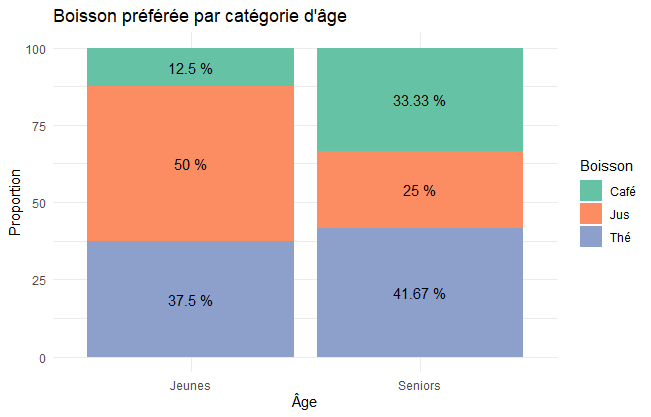
\includegraphics[scale=0.7]{lien_quali_prop.png}
	\end{center}
\end{frame}

%------------------------------------------------
%	NEW SLIDE
%------------------------------------------------
\begin{frame}
\textcolor{nyubluedarker}{\faLightbulb[regular]} Intuitivement, les variables $x$ et $y$ sont \textbf{indépendantes} si les profils-lignes \emph{(et les profils-colonnes)} sont identiques :
	\begin{align*}
	 & \forall k \in \{1,\ldots,K\}, \ \dfrac{n_{1,k}}{n_{1,\cdot}} = \dfrac{n_{2,k}}{n_{2,\cdot}}=\dots = \dfrac{n_{J,k}}{n_{J,\cdot}} \\
	\Longrightarrow & \forall j \in \{1,\ldots,J\}, \ \forall k \in \{1,\ldots,K\}, \ \dfrac{n_{j,k}}{n_{j,\cdot}}=\dfrac{n_{\cdot,k}}{n}.
	\end{align*}
\textcolor{nyubluedarker}{\faLightbulb[regular]} L'\textbf{indépendance empirique} des variables $x$ et $y$ se traduit donc par
	\[
	\boxed{\forall j \in \{1,\ldots,J\}, \ \forall k \in \{1,\ldots,K\}, \ n_{j,k} = \dfrac{n_{\cdot,k} n_{j,\cdot}}{n}.}
	\]
\end{frame}

%------------------------------------------------
%	NEW SLIDE
%------------------------------------------------
\begin{frame}
	\begin{block}{\textbf{$\chi^2$ d'écart à l'indépendance}}
	On appelle lien du $\chi^2$ entre les variables $x$ et $y$ l'indice positif
		\[
		\chi^2 = \sum_{j=1}^J \sum_{k=1}^K \dfrac{\left(n_{j,k} - \frac{n_{j,\cdot}n_{\cdot,k}}{n} \right)^2}{\frac{n_{j,\cdot}n_{\cdot,k}}{n}}.
		\]
	\end{block}
	
	\begin{exampleblock}{\textbf{Remarque}}
		\begin{itemize}
		\item La valeur du $\chi^2$ est nulle dans le cas d'indépendance empirique.
		\item Quelle est la borne supérieure de cet indice ?
		\end{itemize}
	\end{exampleblock}
\end{frame}

%------------------------------------------------
%	NEW SLIDE
%------------------------------------------------
\begin{frame}
	\begin{alertblock}{\textbf{Propriété}}
	On a 
		\[
		\chi^2 \leqslant n \times \min \left( J-1,K-1 \right).
		\]
	\end{alertblock}
	
	\vfill
	
	\begin{block}{\textbf{Lien entre les deux variables}}
	On peut mesurer le lien entre les variables $x$ et $y$ avec la proportion
	\[\dfrac{\chi^2}{n\times \min (J-1,K-1)}.\]
	\end{block}
\end{frame}

%------------------------------------------------
%	NEW SLIDE
%------------------------------------------------
\begin{frame}
	\begin{exampleblock}{\textbf{Exemple}}
	Reprenons l'exemple des boissons.
		\begin{scriptsize}
		\begin{center}
		\begin{tabular}{|c|c|c|c|c|}
		\hline
		\diagbox[height=0.5cm]{$x$ \ }{$y$} & Café & Thé & Jus de fruit & Total \\ \hline
		Jeunes & 5 & 15 & 20 & 40 \\ \hline
		Seniors & 20 & 25 & 15 & 60 \\ \hline
		Total & 25 & 40 & 35 & 100\\ \hline
		\end{tabular}
		\end{center}
		\end{scriptsize}
		
		On a ici
			\[
			\chi^2 = \dfrac{\left(5 - 40\times 25/100\right)^2}{40\times 25/100}+\dots + \dfrac{\left(15-60\times 35/100 \right)^2}{60\times 35/100} \approx 32.5
			\]
		et la proportion de lien des deux variables est donnée par
			\[
			\dfrac{\chi^2}{100} \approx 0.325.
			\]
	\end{exampleblock}
\end{frame}

%------------------------------------------------
%	NEW SLIDE
%------------------------------------------------
\begin{frame}
	\begin{block}{\textbf{A retenir}}
		\begin{itemize}
		\item Représentations graphiques \emph{(variable qualitative, variables quantitative)}.
		\item Indicateurs statistiques pour une variable quantitative \emph{(de position, de dispersion, détermination d'outliers)}.
		\item Lien entre variables quantitatives \emph{(coefficient de corrélation)}.
		\item Lien entre une variable quantitative et une variable qualitative \emph{(décomposition de la variance)}.
		\item Lien entre deux variables qualitatives \emph{(profils lignes/colonnes, coefficient du $\chi^2$)}.
		\end{itemize}
	\end{block}
\end{frame}

\end{document}